\section{Zielsetzung}
\noindent In diesem Versuch werden grundlegende Gesetzmäßigkeiten der Strahlenoptik, die aus den Phänomenen der Reflexion, Brechung und Beugung von Licht resultieren, untersucht.
    

\section{Theorie}
\label{sec:Theorie}
Wellen und ihre Ausbreitung werden in der Strahlenoptik mit Lichtstrahlen beschrieben. Da die 
Ausbreitungsgeschwindigkeit und somit auch die lokale Lichtgeschwindigkeit in unterschiedlichen Materialien unterschiedlich ist, entsteht beim 
Übergang von einem Material in ein anderes der Effekt der Brechung. Der Lichtstrahl wird gebrochen und verändert seine Richtung. 
Diese Änderung berechnet dich durch die Beziehung

    \begin{equation}
        \frac{\text{sin}\alpha}{\text{sin} \beta} = \frac{v_1}{v_2} = \frac{n_2}{n_1},
    \end{equation}

    \noindent   hier sind v die Geschwindigkeiten und n die Brechungsindizes in den jeweiligen Materialien. Der Einfallswinkel ist $\alpha$ und der 
    Brechungswinkel $\beta$.

    \begin{figure}[H]
        \centering
        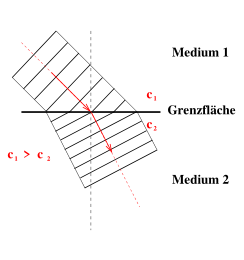
\includegraphics[width=0.3\textwidth]{images/pic1.PNG}
        \caption{Schema der Brechung mit der Beziehung der Ausbreitungsgeschwindigkeiten \cite{400}.}
     \label{fig:brech}
    \end{figure}

    \noindent Werden zwei Materialien verglichen, wird das Material mit höherer Ausbreitungsgeschwindigkeit als optisch dichter bezeichnet und das andere Material als optisch dünner. Bei diesem Experiment ist das optisch dünnere Medium immmer Luft mit n $\approx 1$. Im Bereich der Strahlenoptik bzw. geometrischen Optik sind Lichtstrahlen innerhalb eines homogenen Mediums immer geradlinig und unterschiedliche Strahlen interferieren nicht miteinander.

    \subsection{Reflexion}

        \noindent Wird ein Lichtstrahl an einer ebenen Fläche reflektiert, so ist nach dem Reflexionsgestz der Einfallswinkel $\alpha_1$ gleich dem
        Reflexionswinkel $\alpha_2$. Dies ist schematisch in \autoref{fig:ref} dargestellt.

        \begin{figure}[H]
            \centering
            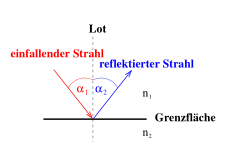
\includegraphics[width=0.4\textwidth]{images/pic2.PNG}
            \caption{Schema zur Reflexion \cite{400}.}
            \label{fig:ref}
        \end{figure}

    \subsection{Brechung}

        \noindent Beim Auftreffen auf ein Medium mit einem anderem Brechungsindex $n$ wird der Lichtstrahl unter einer Richtungsänderung gebrochen (siehe \autoref{fig:brechung}). Diese Brechung erfolgt nach dem Gesetz von Snellius:

        \begin{equation}
            n_1 \text{sin} \alpha = n_2 \text{sin} \beta
        \end{equation}

        \begin{figure}[H]
            \centering
            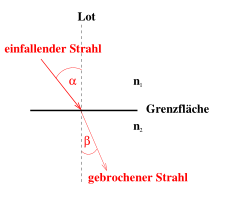
\includegraphics[width=0.4\textwidth]{images/pic3.PNG}
            \caption{Schema zur Brechung \cite{400}.}
           \label{fig:brechung}
        \end{figure}

    \subsection{Reflexion und Transmission}

        \noindent Im Normalfall wird ein Lichtstrahl weder komplett gebrochen noch komplett reflektiert, in der Regel wird ein Teil der Intersität transmitiert und ein Teil gebrochen. In diesem Fall ergeben die Intensitäten dieser beiden Teile wieder die Intensität des einfallenden Strahls.

        \begin{figure}[H]
            \centering
            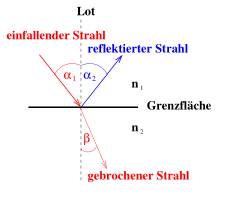
\includegraphics[width=0.4\textwidth]{images/pic4.PNG}
            \caption{Schema zur Reflexion und Transmission \cite{400}.}
            \label{fig:trans}
        \end{figure}

    \subsection{Wellenoptik}
        
        \noindent Die $Strahlenoptik$ kann allerdings nicht alle beobachtbaren Phänomene wie zum Beispiel die Beugung erklären. Um die Beugung zu erklären muss mit der $Wellenoptik$ argumentiert werden.\\
        In diesem Bereich besitzten Wellen eine Frequenz $\nu$, die Ausbreitungsgeschwindigkeit $v$ und somit auch eine Wellenlänge $\lambda$.
        Mehrere Wellen interferieren jetzt miteinander, das bedeutet, dass sich die Gesamtintensität der Wellen an einem Punkt aus der Summe der 
        Einzelintensitäten berechnet (Superpositionsprinzip). Sind unterschiedliche Wellen aus der gleichen Frquenz und dem gleichen Phasengang 
        aufgebaut, erzeugen sie ein so genanntes Interferenzbild. Bei Interferenz wird zwischen konstruktiver und destruktiver Interferenz 
        unterschieden. Haben zwei Wellen gleiche Frequenz, Intensität und genau einen Gangunterschied von $\lambda$/2, so können sie sich 
        komplett auslöschen.\\
        In diesem Versuch wird auch die Beugung an einem Gitter genauer untersucht, es ist wichtig, dass die Dimensionen dess Gitters klein im 
        Vergleich zur Wellenlänge des Lichts sind. Hier besagt das Huygensche Prinzip 'Jeder Punkt einer Welle ist der Ausgangspunkt einer 
        Elementarwelle gleicher Frequenz. Die Einhüllende aller Sekundärwellen stellt zu einem spätere Zeitpunkt die neue Lage der Wellenfront
        dar' \cite{400}.\\
        Ein einfaches Beispiel hierzu ist der Einzelspalt. Trifft monochromatisches Licht, also eine ebene Wellenfront gleicher Phase auf einen Spalt der Breite $a$ wird das Licht nach dem Huygenschen Prinzip in allen Punkten des Spalts gebeugt. Die neuen Wellenfronten 
        haben dann dieselbe Frequenz, eine feste Phasenbeziehung und auf einem Schirm in einem bestimmten Abstand kann ein Interferenzbild gemessen werden. 
        Die Intensitätsmaxima werden dann durch 

        \begin{equation}
            a \, \text{sin} \alpha = k \lambda
        \end{equation}

        \noindent
        berechnet. Hier beschreibt $\alpha$ den Winkel zur geradlinigen Ausbreitung des k'ten Intensitätsmaximums bei einem Einzelspalt der Breite a 
        und einer Wellenlänge $\lambda$.\\
        Analog lässt sich ein Gesetz für ein Gitter aus N-Einzelspalten aufstellen:

        \begin{equation}
            d \, \text{sin} \alpha = k \lambda.
        \end{equation}

        \noindent In dieser Gleichung ist $d$ die Gitterkonstante des gewählten Gitters.
